\documentclass[]{article}
\usepackage[]{amsmath}
\usepackage{listings}
\usepackage{xcolor}
\usepackage{graphicx}
\usepackage{siunitx}
\usepackage{hyperref}
\usepackage{natbib}

\definecolor{codegreen}{rgb}{0,0.6,0}
\definecolor{codegray}{rgb}{0.5,0.5,0.5}
\definecolor{codepurple}{rgb}{0.58,0,0.82}
\definecolor{backcolour}{rgb}{0.95,0.95,0.92}

\lstdefinestyle{mystyle}{
    backgroundcolor=\color{backcolour},
    commentstyle=\color{codegreen},
    keywordstyle=\color{magenta},
    numberstyle=\tiny\color{codegray},
    stringstyle=\color{codepurple},
    basicstyle=\ttfamily\footnotesize,
    breakatwhitespace=false,
    breaklines=true,
    captionpos=b,
    keepspaces=true,
    numbers=left,
    numbersep=5pt,
    showspaces=false,
    showstringspaces=false,
    showtabs=false,
    tabsize=2
}

\lstset{style=mystyle, language=Octave}

\title{From backscatter to suspended sediment concentrations}
\author{Bart Vermeulen}
\setcounter{tocdepth}{2}
\begin{document}
\maketitle
\tableofcontents
\section{Introduction}
In this document first a theoretical overview is given of different methods to compute sediment concentration from backscatter backscatter of ADCPs. Subsequently, a step-by-step guide explains how to perform the calibration using the adcptools.

\section{Calibration methods in general}
\subsection{Theory}
\label{sec:general_theory}
To obtain sediment concentration from the intensity of the echo received by the ADCP, we first want to estimate the backscatter intensity, i.e. the intensity with which sediment reflects incoming sound, since the backscatter intensity directly relates to sediment concentration. 

The backscatter intensity can be computed from the raw echo the instrument receives. The intensity of this echo is determined by the intensity of sound emitted, the spatial spreading, background noise, the directional sensitivity of the transducer, the interference of sound near the transducer, the attenuation of sound by water and sediment and the intensity with which the sound is reflected by particles in a volume, the so-called volume backscatter strength.  All of these factors can be determined a-priori, except for the sediment attenuation, since we do not yet know the sediment concentration. Because of this, we start by estimating the backscatter intensity under the assumption that sediment is not inducing any sound attenuation:
\begin{align}
  S_{v,\alpha_s=0}= C + 10\log_{10}\dfrac{(T+273.16)R^2 \psi^2}{LP_\text{T}}  + 2\alpha_\text{w}R + 10\log10\left(10^{\frac{K_\text{c}E}{10}}-10^{\frac{K_\text{c}E_\text{r}}{10}}\right)
\end{align}

The challenge is to find a relation between the backscatter intensity, attenuation, and sediment concentration. Several methods have been proposed to establish such relation, and most involve some kind of calibration using water samples from which mass concentration and sometimes also other sediment characteristics can be estimated.
In this document we will consider two methods. The first, a simpler method, is the so-called power-law method \citep{hoitink2005} and the second, more elaborate method, is the so-called constant grain size distribution method \citep{sassi2012}.
\subsection{How to}
\label{sec:general_howto}
\subsubsection{Backscatter intensity}
For all calibration methods it is necessary to estimate the uncorrected backscatter intensity. In \lstinline!adcptools! this computation is implemented in the \lstinline!ADCP! class. This class requires a structure read by \lstinline!readDeployment! to be constructed, so we start by reading in the necessary data:
\begin{lstlisting}
path='./raw_data/'; % point this to where your data are located
depname='survey'; % deployment name of the data to read
dat=readDeployment(depname,path); % load the data
\end{lstlisting}

Once the data were loaded an \lstinline!ADCP! object can be constructed\footnote{In case of a vessel mounted deployment you may consider using the \lstinline!VMADCP! class instead, for added functionaly specific for vessel mounted deployments (e.g. ship velocity computations, depth computations, GPS data processing). This will not affect acoustic computations.}:
\begin{lstlisting}
A=ADCP(dat); % Construct ADCP object
\end{lstlisting}


The \lstinline!ADCP! class is able to compute the uncorrected backscatter intensity, but before doing so it is important to check, and possibly change a number of properties of the object.
The raw PD0 data that has been read does not always allow to determine the kind of ADCP the data was collected with. The type of ADCP is important to correctly estimate all instrument constants for Equation~\ref{eq:powerlaw}. The type of ADCP can be set with the \lstinline!type! property of the \lstinline!ADCP! object. The value is an enumeration of class \lstinline!ADCP_Type!: 
\begin{lstlisting}
A.type=ADCP_Type.Monitor; % set correct type of ADCP, change to your own settings
\end{lstlisting}
A list of ADCP types is obtained by typing \lstinline!ADCP_Type.! and then pressing the TAB button.

Then it is important to check the water properties, needed for the acoustics computations. These can be checked by getting the \lstinline!acoustics.Water! object contained in the \lstinline!water! property. The salinity\footnote{Salinity is specified in ppm, roughly PSU*1000} and temperature should meet conditions during data collection: 
\begin{lstlisting}
plot(A.water.salinity)
figure
plot(A.water.temperature)
\end{lstlisting}
These properties are read from the ADCP raw data.

Finally it is important to check the transducer characteristics. These are obtained with the \lstinline!transducer! property. Make sure, \lstinline!depth!, \lstinline!radius! and \lstinline!frequency! are correct.

Now it is possible to obtain the uncorrected backscatter intensity $S_{v,alpha_s=0}$:
\begin{lstlisting}
sv1=A.backscatter(:,:,1); % backscatter intensity as measured in the first acoustic beam
imagesc(sv1) % plot the backscatter intensity
\end{lstlisting}

The backscatter intensity involves the computation of many instrument properties. All relevant properties can be found in the help of the \lstinline!ADCP! class, under the header \lstinline!Backscatter!.

\subsubsection{Water samples and calibration objects}
For all calibration it is necessary to specify water samples and ADCP data, and all calibration are expected to produce suspended sediment mass concentration. Also, for all calibrations it will be necessary to match ADCP and water samples data. All this functionality is implemented in the \lstinline!acoustics.Sv2SSC! abstract base class \footnote{An abstract base class is a class that implements some basic functionality, common for all subclasses. The term abstract refers to the fact that the class can not be used directly, since it requires additional implementation to function properly (see the methods defined as Abstract in the code, these lack implementation). Implementation of Abstract methods is done in so-called concrete subclasses that can actually be used. For this reason an abstract base class can also be seen as a sort of template or interface}. This means that the class cannot be used directly, but all different calibrations will derive from this base class, and share its properties and methods.

Water samples are defined with the \lstinline!acoustics.WaterSample! class. For each water sample collected, an object is made. E.g. if we collected 10 water samples we will create an array of 10 objects:
\begin{lstlisting}
samples(10)=acoustics.WaterSample; % Construct 10 water samples
\end{lstlisting}
Now for each of the samples it is possible to define the properties. The most important are the \lstinline!time!, needed to match with ADCP time. Note that if the time zone differes between ADCP and Water Samples, the time zone must be specified in the \lstinline!time! property (see help on how to do that) and in the \lstinline!timezone! property of the ADCP. Then the \lstinline!distance! property defines the vertical distance between transducer and water sample. \lstinline!mass_conentration! defines the mass concentration. It is also possible to assign a grain size distribution with the \lstinline!distribution! property. Check the help of the property to see how to define that. This allow to estimate backscatter and attenuation based on the grain size distribution. This is usually less reliable than the results from the calibration. 

Once the water samples are defined, they can be assigne to a calibration object:
\begin{lstlisting}
S=Sv2SSC_Power; % Need to use a derived class for the demo, but code holds for any calibration
S.samples=samples; % Define the water samples
S.adcp=A; % Define the ADCP class for calibration
\end{lstlisting}
We also assigned the ADCP object. The last property that must be defined is the averaging duration. This is a \lstinline!duration! object:
\begin{lstlisting}
S.duration=duration(0,3,0); % Set the averaging duration to 3 minutes
\end{lstlisting}
The methods defined in the \lstinline!acoustics.Sv2SSC! class can now be used to get the right backscatter intensity matching with the samples with \lstinline!sv_for_calibration! method. This returns an averaged backscatter intensity for every water sample collected. A \lstinline!plot! method, allows to easily inspect whether the mass concentrations and the backscatter intensitys show a reasonable relation:
\begin{lstlisting}
plot(S) % plot the backscatter intensity vs. the mass concentration for the given water samples
\end{lstlisting}

Finally the class defines the method \lstinline!mass_concentration! that can be used to estimated mass concentration from ADCP backscatter. This function is implemented differently for each method, but the use is the same. If no argument is passed, the concentration is determined for the backscatter of the ADCP object used for calibration. Alternatively an array of backscatter intensitys can be passed to the method and the corresponding mass concentrations are returned:
\begin{lstlisting}
ssc=S.mass_concentration; % get the mass concentration for the ADCP used in the calibration
imagesc(ssc(:,:,1)) % plot the sediment concentration based on the first acoustic beam
\end{lstlisting}

Each calibration will define its own properties and method specific for that calibration. Detailes are given below.
\section{The power law method}
\subsection{Theory}
The power law method assumes a relation between suspended sediment concentration $M$ and the backscatter intensity $S_v$:
\begin{equation}
  \frac{M}{M_0}=10^{aS_{v,\alpha_s=0}+b}
  \label{eq:powerlaw}
\end{equation}
with $M_0$ equal to \SI{1}{\milli\g\per\liter}. The values for $a$ and $b$ are obtained by regression between $\log(M/M_0)$. Water samples are used to estimate the two parameters. Once the two parameters are estimated, mass concentration is easily obtained using Equation~\ref{eq:powerlaw}.

\subsection{How to}
The class to perform the power law calibration is the \lstinline!acoustisc.Sv2SSC_Power! class. The class can be constructed as explained in section~\ref{sec:general_howto}. The class defines additional methods specific to this calibration method. The \lstinline!calibrate_a_b! method performs the regression as explained above and outputs the parameters $a$ and $b$. It can also return the standard deviation of the two estimated parameters (see help of the class). 

Eventually backscatter intensity can be converted to mass concentration with the \lstinline!mass_concentration! method as explained in section~\ref{sec:general_howto}

\section{The constant grain size distribution method}

\subsection{Theory}
The method proposed by \citet{sassi2012} assumes a constant grain size distribution over the measuring range, which means that the specific attenuation and specific backscatter intensity are constant over the measuring range. This means that this method should be particularly applicable in regions where no major grain size distribution changes are expected over the measured range.

The method consists of calibrating two parameters:
\begin{itemize}
  \item $b$ which expresses the relation between sediment backscatter and mass concentration (similar to the $b$ in the power law method)
  \item $\xi_s$ attenuation per unit concentration (specific attenuation)
\end{itemize}
The first parameter $b$ requires a sample collected very close to the ADCP transducer (but outside of the blanking distance), such that we can assume the effect of attenuation to be negligible.
To estimate the second parameter $\xi_s$ another sample can be collected at a larger depth. This sample should preferably be near the last cell of the ADCP. More samples can be collected at different depths to estimate depth variations in $\xi_s$ or to increase the statistical significance of the estimates.


\subsubsection{Part 1: estimate $b$}
With the uncorrected backscatter $S_{v,alpha_s=0}$ (see section~\ref{sec:general_theory} and sediment concentration measurements near the transducer the first calibration step can be performed in which we try to estimate the parameter $b$ from equation 14 of \citet{sassi2012}:
\begin{align}
  K(R_\text{ref})=a\beta(\tilde{R}_\text{ref})^b
\end{align}
where $R_\text{ref}$ is the range where the water samples were collected, $K=\beta/M_\text{s}$, $\beta=10^{S_{\text{v,}\alpha_\text{s}=0}/10}$, $M_s$ is the measured sediment concentration, $a=1/[M_\text{s}]$ (i.e. the inverse of the sediment concentration unit). 
Once we obtained this estimate we preceed with an estimate of the specific attenuation

\subsubsection{Part 2: estimate $\xi_s$}
The last step of the calibration will yield $\xi_s$ using equation 15 from \citet{sassi2012}:
\begin{align}
  \gamma_e=\dfrac{\ln(10)}{5}\xi_s=\dfrac{K(R_1)-\dfrac{\beta(R_2)}{M_s(R_2)}}{\int_{R_1}^{R_2}\beta(r)\;\text{d}r}
\end{align}
For this step we will need two samples. The first can be a sample used during the first calibration step, The second should preferably be near the end of the ADCP measuring range. This last step can be done with different combinations of samples to obtain $\xi_s$ varying over depth. It is recommended to use several samples to estimate $\xi_s$ and select a representative estimate. \citet{sassi2012} used the mode of all estimates in the dataset.


\subsubsection{Estimate sediment concentration}
The last step is to use the calibration to compute sediment concentration profiles for the measured ADCP data.
This is done by using equation 13 from \citet{sassi2012}:
\begin{align}
  M_s(R)=\dfrac{\beta(R)}{K(R_\text{ref})-\gamma_e\int_{R_\text{ref}}^R\beta(r)\;\text{d}r}
\end{align}








%Next to these basic parameters, there are a number of additional parameters that can be calibrated:
%\begin{itemize}
%  \item The RSSI scale factor $K_c$ (dB/count) and the calibration coefficient $C$ are both instrument specific constants that can be calibrated when water samples are available at the start of the ADCP measuring range and with known grain size distribution.
%  \item The density of the backscattered particles $\rho_s$ can be calibrated when both mass concentrations (e.g. from filtration) and volume concentration (e.g. from Malvern or LISST) are available
%\end{itemize}
%
%To estimate parameters $b$ and $\xi_s$ we will need:
%\begin{itemize}
%  \item Water samples near the transducer, but far enough to be in the detection range of the ADCP (outside the blanking distance)
%  \item Water samples deeper in the water column.
%    \begin{itemize}
%      \item At least one or more at the end of the ADCP measuring range.
%      \item Optionally samples at more depths if variations in $\xi_s$ are expected over depth (e.g. changing grain size distribution)
%    \end{itemize}
%  \item Exact depth the samples were taken
%  \item Time the samples were taken
%  \item ADCP echo intensity values from the ADCP collected at the time the sample was taken (2-3 minutes of data are recommended)
%  \item Transducer characteristics
%    \begin{itemize}
%      \item Operating frequency
%      \item Diameter
%      \item RSSI scale factor $K_c$ (dB/count, ADCP characteristic which can be obtained from the manufacturer, calibrated in a lab with a hydrophone or estimated if grain size distributions have been determined.)
%      \item RSSI in a bucket $E_r$ (counts, background noise, see PT3 command on RDI ADCPs)
%      \item Calibration coeff $C$ (dB, instrument specific constant, can be obtained from manufacturer or estimated if grain size distributions have been determined.)
%    \end{itemize}
%  \item Water characteristics
%    \begin{itemize}
%      \item Temperature
%      \item Salinity (For stratified conditions CTD data are needed)
%    \end{itemize}
%  \item Depth of the ADCP transducer (insteekdiepte)
%\end{itemize}
%
\subsection{How to}
To perform the constant grain size distribution calibration the class \lstinline!acoustics.Sv2SSC_ConstantGSD! can be used. In addition to specifying the \lstinline!samples! and \lstinline!adcp! properties, this calibration also requires to set two additional properties. The first is the \lstinline!reference_idx! and the second is the \lstinline!attenuation_idx!. These properties specify the samples that will be used as reference samples (to estimate $b$) and the once to be use for the specific attenuation estimates (to estimate $\xi_s$). The can e.g. be specified based on the distance:
\begin{lstlisting}
dist=[S.samples.distance]; % get the vertical distance from the tranducer to the samples
S.reference_idx=find(dist<5.5); % select the close ones as reference samples
S.attenuation_idx=find(dist>5.5); % and the other ones as attenuation samples
\end{lstlisting}
Now the two parameters can be estimated using the \lstinline!calibrate_b_gamma! method:
\begin{lstlisting}
[b, stdb, gamma_e, xi_e]=S.calibrate_b_gamma();
\end{lstlisting}
The \lstinline!b! parameter is a single value based on the reference samples. \lstinline!stdb! holds the standard deviation of $b$. \lstinline!gamma_e! holds the estimated $\gamma$ values for the attenuation samples. It will have one value per sample. Since the spread in these values can be rather large, it is good to manually inspect these values and choose a suitable value to work with. In \citet{sassi2012} the mode of these values was chosen. The \lstinline!xi_e! output holds the $\xi_s$ values, that are closely related to the $\gamma$ values \citep[see equation 12, ][]{sassi2012}. 

The last step in the calibration is to obtain the sediment concentrations. this is done using the \lstinline!mass_concentration! method as explained before. For options in the used of this method see the help of the method.


%The computations will be performed in the following order:
%\begin{enumerate}
%  \item Compute $\rho_s$, if volume and mass concentration are available for sample (optional)
%  \item Calibrate $K_c$ and $C$ if GSD is available for samples collected near the transducer (optional)
%  \item Calibrate $b$ and $\xi_s$ from mass concentration samples
%  \item Compute mass concentration profiles for volume backscatter intensity
%\end{enumerate}
%
%\subsection{Calibration of $\rho_s$ (optional)}
%$\rho_s$ is easily estimated when mass concetration $M_\text{s}$ and volume concentration $C$ are available:
%\begin{equation}
%  \rho_s=\dfrac{M_s}{C}
%\end{equation}
%Specifying the \lstinline!volume_concentration! and \lstinline!mass_concentration! properties of the \lstinline!acoustics.WaterSample! class will automatically compute the density given in the \lstinline!sediment_density! property.
%\subsection{Calibration of $K_c$ and $C$ (optional)}
%The basis for this calibration is that we can compute the volume backscatter intensity $S_v$ both from the GSD and sediment concentration and from the ADCP backscatter. Than we can estimate $K_c$ and $C$ as unknowns.
%The first step is to estimate the $k_s^2$. This is based on the mean backscatter cross-section $\langle\sigma_{bs}\rangle$ that is computed from the form function and the GSD:
%\begin{align*}
%  S_v=&10\log_{10}(k_s^2M_s)\\
%  k_s^2=&\dfrac{3}{16\pi\rho_s}\dfrac{\langle a_s^2 f^2 \rangle}{\langle a_s^2\rangle}\\
%\end{align*}
%In \texttt{adcptools} we will first need to create an \texttt{acoustics.PisontTransducer} object.
%\begin{lstlisting}[language=Octave]
%pt=acoustics.PistonTransducer;
%\end{lstlisting}
%Than we set the right frequency and transducer diameter:
%\begin{lstlisting}[language=Octave]
%pt.frequency=1228.8e3; %for a 1200 kHz ADCP
%pt.radius=0.027; % radius of 2.7 cm
%\end{lstlisting}
%The \texttt{acoustics.PistonTransducer} object also contains a \texttt{Water} object that is used to compute the speed of sound in water given temparature, salinity and pH.
%
%Now we can construct an \texttt{acoustics.GrainSizeDistribution} object and assign fractions and diameters:
%\begin{lstlisting}
%gs=1e-6*[0.01 0.011482 0.013183 0.015136 0.017378 0.019953 0.022909 0.026303 0.0302 0.034674 0.039811 0.045709 0.052481 0.060256 0.069183 0.079433 0.091201 0.104713 0.120226 0.138038 0.158489 0.18197 0.20893 0.239883 0.275423 0.316228 0.363078 0.416869 0.47863 0.549541 0.630957 0.724436 0.831764 0.954993 1.096478 1.258925 1.44544 1.659587 1.905461 2.187762 2.511886 2.884031 3.311311 3.801894 4.365158 5.011872 5.754399 6.606934 7.585776 8.709636 10 11.481536 13.182567 15.135612 17.378008 19.952623 22.908677 26.30268 30.199517 34.673685 39.810717 45.708819 52.480746 60.255959 69.183097 79.432823 91.201084 104.712855 120.226443 138.038426 158.489319 181.970086 208.929613 239.883292 275.42287 316.227766 363.078055 416.869383 478.630092 549.540874 630.957344 724.43596 831.763771 954.992586 1096.478196 1258.925412 1445.439771 1659.586907 1905.460718 2187.761624 2511.886432 2884.031503 3311.311215 3801.893963 4365.158322 5011.872336 5754.399373 6606.93448 7585.77575 8709.6359 10000];
%fract=.01*[0 0 0 0 0 0 0 0 0 0 0 0 0 0 0 0 0 0 0 0 0 0 0 0 0 0 0 0.178333 0.301668 0.385886 0.445449 0.469272 0.467858 0.449735 0.42987 0.422813 0.441772 0.49676 0.595676 0.749952 0.974694 1.284648 1.689853 2.185246 2.760847 3.378964 4.007627 4.583791 5.068609 5.405399 5.574199 5.560831 5.378561 5.063955 4.655804 4.211591 3.768856 3.366553 3.018285 2.730382 2.494196 2.29615 2.120405 1.951593 1.781102 1.601525 1.414943 1.222138 1.035633 0.861343 0.712813 0.587049 0.47997 0.380193 0.279534 0.188959 0.073695 0.01502 0 0 0 0 0 0 0 0 0 0 0 0 0 0 0 0 0 0 0 0 0 0];
%gsd=acoustics.GrainSizeDistribution(gs,fract);
%\end{lstlisting}
%Now we can compute all kinds of acoustic characteristics of the sediment. A quick view can be obtined by running:
%\begin{lstlisting}
%gsd.plot_all(pt)
%\end{lstlisting}
%This will produce a figure similar to figure~\ref{fig:gsd}.
%\begin{figure}[h]
%  \centering
%  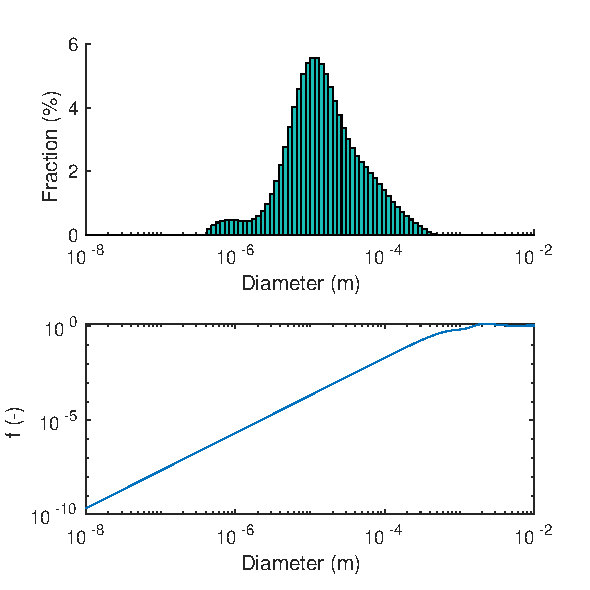
\includegraphics{gsd.pdf}
%  \caption{Example of grain size distribution and the corresponding form function}
%  \label{fig:gsd}
%\end{figure}
%The $k_s^2$ is now easily obtained as:
%\begin{lstlisting}
%ks2=gsd.ks_squared(pt, rhos);
%\end{lstlisting}
%Now that the $k_s^2$ is computed the $S_v$ is easily obtained having the sediment concentration.
%
%\subsection{Calibration}
%For the calibration we will need to first estimate the backscatter intensity under the assumption that there is no sediment attenuation $S_{v,\alpha_s=0}$:
%\begin{align}
%  S_{v,\alpha_s=0}= C + 10\log_{10}\dfrac{(T+273.16)R^2 \psi^2}{PL_\text{T}}  + 2\alpha_\text{w}R + 10\log10\left(10^{\frac{K_\text{c}E}{10}}-10^{\frac{K_\text{c}E_\text{r}}{10}}\right)
%\end{align}
%This computation can be performes with the \texttt{svADCP.m} script. This script requires as input the adcp structure (read by \texttt{readADCP.m}) and a \texttt{acoustics.PisontTransducer} object. Please note that this equation is the equation as proposed by Gostiaux and van Haren (2010), in which the last term differs from Deines (1999).
%
%
\section{In depth acoustics}
Next to the calibration methods to obtain Suspended sediment concentrations there are a number of additional acoustic computations that are supported in \lstinline!adcptools!. The most important ones are perfromed in the \lstinline!acoustics.PistonTransducer!, the \lstinline!acoustics.Water! class and the \lstinline!acoustics.GrainSizeDistribution! class.
\subsection{Water}
Since we are dealing with sound propagation in water, it is important to estimate the acoustic properties of water. The class currently supports the estimate of the density $\rho$, dynamic $\mu$ and kinematic $\nu$ viscosity and the speed of sound $c$. The first three properties depend on temperature and salinity, and the last one (the speed of sound) also depends on the depth. The class \lstinline!acoustics.Water! supports all these computations. 

You can set the following properties of the \lstinline!acoustics.Water! class:
\begin{itemize}
  \item \lstinline!temperature!: Temperature in degrees Celsius
  \item \lstinline!salinity!: Salinity in parts per million (ca. psu/1000)
  \item \lstinline!pH!: pH of water
\end{itemize}
All of these properties can have any size, as long as the dimensions of the arrays can be combined in an elementwise manner.

The following properties can be obtained from the object:
\begin{itemize}
  \item \lstinline!density!: density of water in \si{\kilo\gram\per\cubic\meter} \citep[equation 8, ][]{sharqawy2010}
  \item \lstinline!dyn_viscosity!: dynamic viscosity of water \si{\kilo\gram\per\m\per\s} \citep[equations 22 and 23, ][]{sharqawy2010}
  \item \lstinline!kin_viscosity!: kinematic viscosity of water \si{\m\squared\per\s} (from the two above)
  \item \lstinline!speed_sound!: speed of sound \si{\m\per\s} \citep[equation 3.3.3, ][]{medwin1998}
\end{itemize}
\subsection{Transducer}
Different types of transducers exist. ADCPs generally use piston transducers, although recently also phased array transducers are being used. The last type of tranducers is currently not supported. Computations related to piston transducers are implemented in the \lstinline!acoustics.pistonTransducer! class. Properties that can be set on this class are:
\begin{itemize}
  \item \lstinline!radius!: Radius of the transducer in \si{\m}
  \item \lstinline!freqeuncy!: Frequency of the transducer in \si{\hertz}
  \item \lstinline!depth!: Depth of the transducer in \si{\m}
  \item \lstinline!water!: \lstinline!acoustics.Water! object specifying water properties 
\end{itemize}
Also here, the properties can be of any size (except the water properties, which is scalar, but the properties of water can be of any size), as long as elementwise operations can be done on them.

The following methods are defined:
\begin{itemize}
  \item \lstinline!wavelength! - wavelength in m
  \item \lstinline!wavenumber! - angular wave number of the sound waves in 1/m
  \item \lstinline!nearfield! - range of near field in m
  \item \lstinline!angularfreq! - angular frequency of the sound waves in rad/s
  \item \lstinline!attenuation! - sound attenuation caused by water in dB/m
  \item \lstinline!attenuation_e! - sound attenuation caused by water in 1/m (neper)
  \item \lstinline!speedsound! - speed ouf sound in water in m/s
  \item \lstinline!directivity! - Directivity of the emitted sound (neper)
  \item \lstinline!dir_response! Directional response (dB) of the transducer
  \item \lstinline!near_field_correction! - Compute the near field correction factor
  \item \lstinline!side_lobes! - Compute angle of transmitted side lobes
  \item \lstinline!zeros! - Compute angle (radians) where no sound it transmitted
  \item \lstinline!plot! - Plot the directional response of the transducer
  \item \lstinline!plot_3d! - Make a 3D plot of the directional response
\end{itemize}
\bibliographystyle{lit}
\bibliography{lit}


\end{document}
